\section{Aufbau und Durchführung}
\label{sec:Aufbau}
\subsection{Aufbau}
\subsubsection{Aufbau zur Bestimmung des Schumbmodules}
Zur Überprüfung der Theorie wird experimentell der Schubmodul $G$  eines Torsionsdrahtes bestimmt.
Hierzu wird dieser Draht aufgehangen, wobei das obere Ende fest an einem Justierrad eingespannt und das untere Ende an einer Kugel befestigt ist.
Durch kurzzeitiges Auslenken aus der Ruheposition mithilfe des Justierrades kann der Torsionsdraht in eine, für kleine Winkel, harmonische Rotationsschwingung versetzt werden.
Deswegen werden im Folgenden nur Auslenkungen im Bereich $\leq \SI{40}{\degree}$ betrachtet.
Der Aufbau ist in Abbildung \ref{fig:d1} skizziert.
\begin{figure}[H]
  \centering
  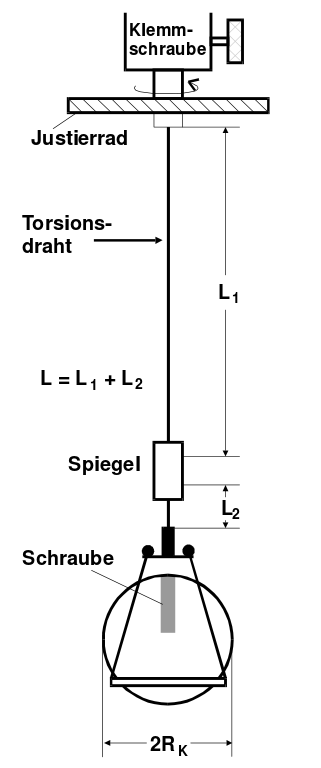
\includegraphics[height=12cm]{aufbau1.png}
  \caption{Messapparatur zur Bestimmung des Schubmoduls eines Torsionsdrahtes. \cite{sample}}
  \label{fig:d1}
\end{figure}
Zwischen dem Torsionsdraht und der Kugelaufhängung befindet sich ein Spiegel, welcher für die Messung der Periodendauer $T$ der Schwingung benötigt wird.
Wie in Abbildung \ref{fig:d2} dargestellt, wird ein Lichtstrahl mithilfe eines Spaltes und einer Sammellinse fokussiert und in Höhe des Spiegels auf den Torsionsdraht gerichtet.
\begin{figure}[H]
  \centering
  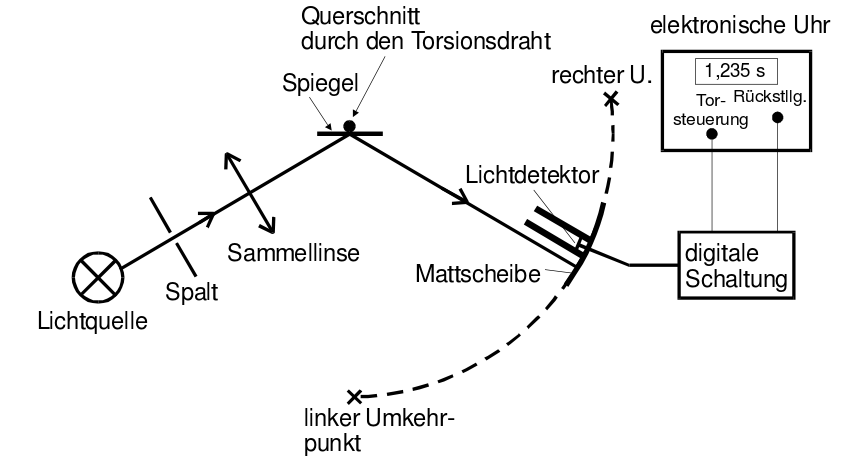
\includegraphics[height=6cm]{aufbau2.png}
  \caption{Bestimmung der Periodendauer $T$ der Schwingung des Torsionsdrahtes mithilfe eines Lichtdetektors. \cite{sample}}
  \label{fig:d2}
\end{figure}
Durch den sich mitrotierenden Spiegel wird der Strahl auf eine Photodiode geworfen.
Somit kann eine bestimmte, feste Auslenkung des Drahtes anhand eines elektrischen Stromes registriert werden.
Um nun eine Periodendauer der Schwingung zeitlich zu bestimmen, wird das elektronische Signal so umgewandelt, dass es mithilfe von digitalen TTL-Bausteinen verarbeitet werden kann.
Sobald die Schwingung eine Phase das erste Mal durchläuft, wird ein erster Lichtstrahl registiert.
Dieser Impuls dient als Startzeitpunkt der Messung.
Nach der Umkehrung der Bewegung durchläuft der Lichtstrahl den Sensor das zweite Mal, dieser Impuls soll ohne Bedeutung sein.
Schlussendlich durchläuft der Lichstrahl den Sensor ein drittes Mal, die Schwingung befindet sich wieder in der gleichen Phase wie zum Anfang und hat eine gesamte Periodendauer durchlaufen.
Dieser dritte Impuls wird dementsprechend als Endzeitpunkt der Messung verwendet.
Mithilfe der TTL-Bausteine, insbesondere eines RS-Flip-Flops und einer monostabilen Kippstufe, wird eine Schaltung so realisiert, dass zwischen dem Startimpuls sowie Endimpuls kontinuirliche Zeitimpulse an eine elektronische Uhr geliefert werden.
An dieser kann somit die Periodendauer abgelesen werden.\\
\subsubsection{Aufbau zur Bestimmung des magnetischen Momentes eines Permamagneten bzw. des Erdmagnetsfeldes}
In der aufgehangenen Kugel befindet sich ein fest eingebauter Permanentmagnet.
Dieser kann durch das Drehen in der Kugel der Versuchsdurchführung entsprechend ausgerichtet werden.
Zudem befindet sich um die aufgehängte Kugel ein Helmholtzspulenpaar, welches ein annähernd homogenes Magnetfeld erzeugen kann.
Die Stärke des Magnetfeldes kann durch das Justieren der Stromstärke eingestellt werden.

\subsection{Durchführung}
Zunächst wird die Länge $l$ des genutzen Torsionsdrahtes mithilfe eines Bandmaßes sowie dessen Durchmesser $d$ mithilfe einer Miktrometerschraube bestimmt.
Hierzu werden jeweils drei beziehungsweise fünf Messungen durchgeführt.
Zudem wird der Abstand vom Reflexionsspiegel zur Kugelaufhängung drei mal gemessen.
Die weiteren Eigenschaften wie Kugelmasse $m_k$, Kugeldurchmesser $d_k$ sowie Trägheitsmoment der Kugelhalterung $I_h$ werden am Versuchsaufbau abgelesen.
Ebenso werden die Eigenschaften des Helmholtzspulenpaars wie Windungszahl $n$, Radius $r_s$ sowie Maximalstrom abgelesen.\\
Zudem wird der zuvor defekte Versuchsaufbau in einer heroischen Tat durch das Neujustieren des Lichtdetektors wieder in den Zustand der Funktionsfähigkeit gebracht.
Eine Heldentat, von der noch Generationen von Physikern erzählen werden.\\
\subsubsection{Bestimmung des Schubmoduls}
Zunächst wird der Schumodul anhand der Periodendauer $T$ bestimmt.
Die Kugel wird so positioniert, dass der Stabmagnet vertikal ausgerichtet ist und das Erdmagnetefeld einen mininmalen Einfluss auf die Messung hat.
Mithilfe des Justierrades wird der Aufbau zu Schwingungen angeregt.
Es werden die Periodendauern für zehn Messungen notiert.
\subsubsection{Bestimmung des Erdmagnetsfeldes}
Es soll nun anhand der veränderten Periodendauer $T_2$ auf die Stärke des Erdmagnetsfeldes geschlossen werden.
Der Stabmagnet wird in Nord-Süd-Richtung ausgerichtet, dementstprechend ist der Einfluss des Erdmagnetsfeldes maximal.
Auch hier wird das System zu Schwingungen angeregt, es werden die Periodendauern für zehn Messungen notiert.
\subsubsection{Bestimmung des magnetischen Moments eines Permanentmagneten}
Im letzten Versuchsaufbau wird die Helmholtzspule eingeschaltet und die Kugel so ausgerichtet, dass der Permanentmagnet in seiner Ruhestellung parallel zu den Feldlinien des Magnetfeldes der Spule steht.
Für fünf verschiedene Stromstärken, bzw. verschiedene Magnetfeldstärken, werden jeweils fünf Messungen der Periodendauer durchgeführt.
